\chapter{Js foundation}

\section{JavaScript Engine}

    JavaScript (\acrshort{js}) engine is a translator between \textit{\acrshort{js} language} and \textit{computer native language} - 0,1  \cite{JavaScriptEngineImage2020}.
    There are tons of \acrshort{js} engines \cite{ECMAScriptEngines}. One of the most famous is google V8 engine. 
    The creator of first \acrshort{js} engine is Brendan Eich cofounder of the Mozilla project, the Mozilla Foundation, and the Mozilla Corporation \cite{BrendanEich}.
    
    \begin{figure}[h]
        \begin{center}
            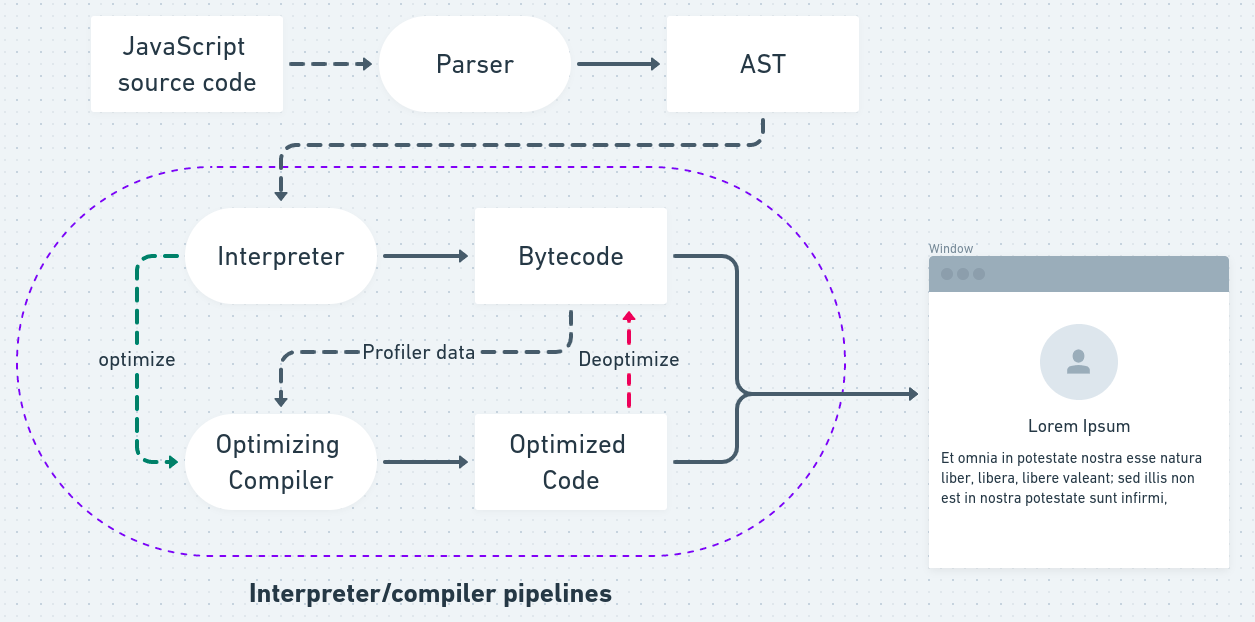
\includegraphics[width=10cm]{01/images/01-js-engine.png}
            \caption[JavaScript engine]{JavaScript engine description  \cite{JavaScriptEngineImage2020}.}
        \end{center}
    \end{figure}

    \subsection{Interpreter vs. compiler}

        \textbf{Interpreter} read and translate code line by line. \acrshort{js} mostly works like interpreted language.
        In computer science, an interpreter is a translator (computer program) that repeatedly reads instructions (one at a time) and translates them to machine code. 
        It then executes instructions written in a programming or scripting language, without requiring them previously to have been compiled into a machine language program. 
        An interpreter generally uses one of the following strategies for program execution:
            \begin{enumerate}
                \item Parse the source code and perform its behavior directly;
                \item Translate source code into some efficient intermediate representation or object code and immediately execute this;
                \item Explicitly execute stored precompiled code made by a compiler which is part of the interpreter system.
            \end{enumerate}

            \textbf{Compiler} is a computer program that translates computer code written in one programming language (the source language) into another language (the target language).
            The name "compiler" is primarily used for programs that translate source code from a high-level programming language to a lower level language (e.g., assembly language, object code, or machine code)
            to create an executable program. There are many types of compilers which produce output in different useful forms. A compiler that can run on a computer whose CPU or operating system is different 
            from the one on which the code it produces will run is called a cross-compiler.
    
    \subsection{Babel and TypeScript}

        \textbf{Babel} is a Javascript compiler that takes your modern JS code and returns  browser compatible JS (older JS code).
        
        \textbf{Typescript} is a superset of Javascript that compiles down to Javascript.

        Both of these do exactly what compilers do: Take one language and convert into a different one!
    
    \section{Inline caching}
    \section{Hidden classes}
    \section{WebAssembly}

    \section{Call Stack and Memory Heap}

        The \textbf(Call stack) shows order of executed commands in JS and primitive variables.
        In a \textbf(stack) data structure that stores information about the active subroutines of a computer program. 
        This kind of stack is also known as an execution stack, program stack, control stack, 
        run-time stack, or machine stack, and is often shortened to just "the stack". 
        Although maintenance of the call stack is important for the proper functioning 
        of most software, the details are normally hidden and automatic in high-level programming languages. 
        Many computer instruction sets provide special instructions for manipulating stacks.

        \textbf{Stack overflow} \acrshort{js} is garbage collected language $\Rightarrow$  automatically clean Call stack. 
        If the program reaches the capacity of the Call Stack (stack data structure), it stops work imediately.

         \begin{lstlisting}[style=ES6, caption={recursive function wich exceed Call stack}]
    // recurisive function
    const inception = () => {
        inception();
    };

    // calling recurisive function with stack overflow
    // RangeError: Maximum call stack size exceeded
    inception();
        \end{lstlisting}

        \textbf(Memory leak) is the unclean (with garbage collector) memory.

        \begin{lstlisting}[style=ES6, caption={Memory leak}]
    let array = []
    for (let i = 5; i>1; i++){
        array.push(i-1);
    }
    // Global variables
    var a = 1;
    var b = 1;
    var c = 1;

    // Event listeners
    var element = document.getElementById('button');
    element.addEventListener('click', onClick);

    // setInterval
    setInterval(() => {})

        \end{lstlisting}

        \begin{figure}[h]
            \begin{center}
                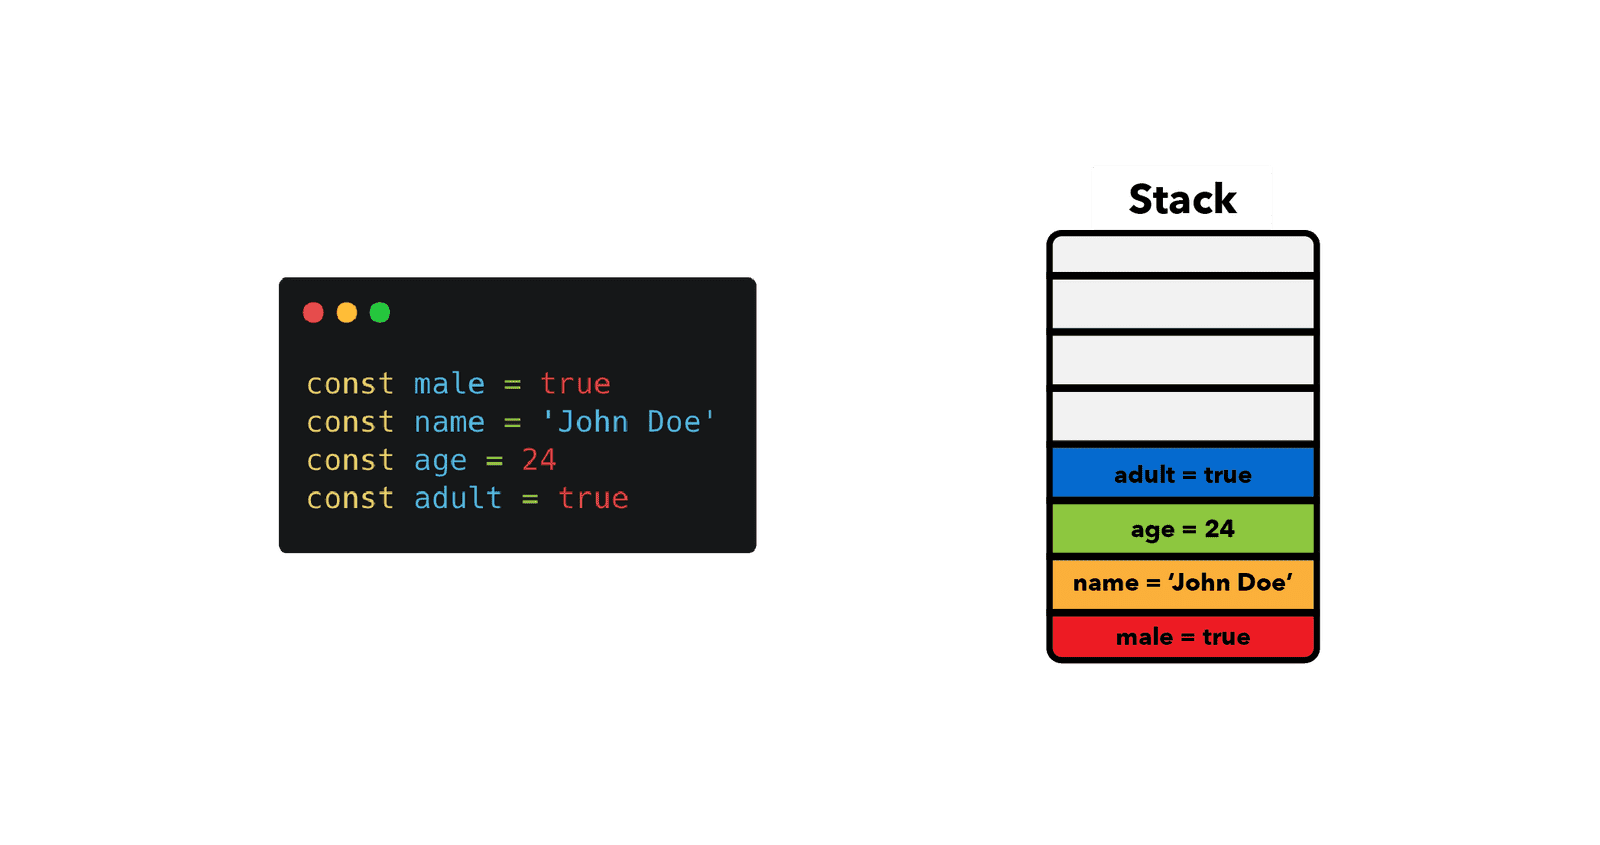
\includegraphics[width=10cm]{01/images/03-stack.png}
                \caption[Call stack]{All the values get stored in the stack since they all contain primitive values \cite{JavaScriptMemoryManagment2020}.}
            \end{center}
        \end{figure}

        The \textbf(Memory Heap) is used for storing dynamic data (objects).
        The memory heap The \textbf(heap) is a different space for storing data where JavaScript stores objects and functions. 
        Unlike the stack, the engine doesn't allocate a fixed amount of memory for these objects. 
        Instead, more space will be allocated as needed. 
        Allocating memory this way is also called dynamic memory allocation.

        \begin{figure}[h]
            \begin{center}
                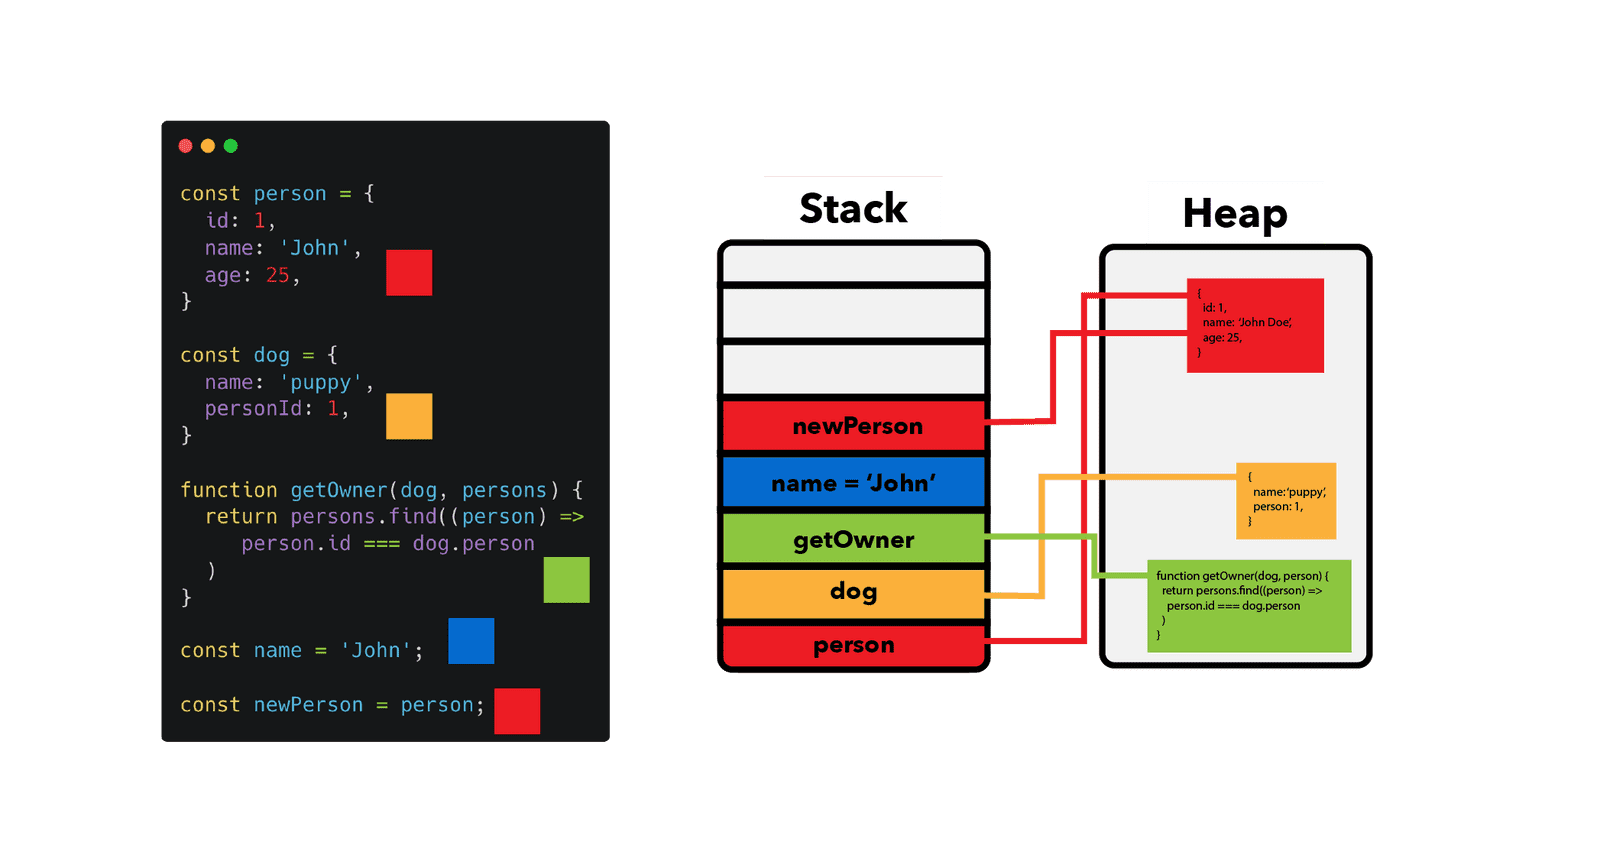
\includegraphics[width=10cm]{01/images/02-stack-heap.png}
                \caption[Memory heap vs Call stack]{In this picture, we can observe how different values are stored. Note how person and newPerson both point to the same object \cite{JavaScriptMemoryManagment2020}.}
            \end{center}
        \end{figure}

    \section{Single-thread}
    \acrshort{js} is a single-threaded programming language. It means only one set of instructions can be executed at time (one Call Stack).
    Because of this \acrshort{js} is synchronous.

    \begin{figure}[h]
        \begin{center}
            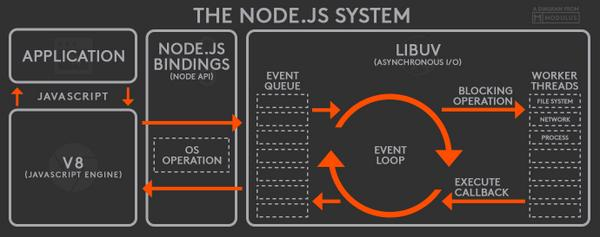
\includegraphics[width=10cm]{01/images/04-single-thread.jpeg}
            \caption[Single thread]{Single thread architecture}
        \end{center}
    \end{figure}

    \section{Runtime}

    \textbf(webAPI) -> provided by web browser ->  (window) -> fetch() -> make http calls

    \section{Node.js}

    is \acrshort{js} \textbf{runtime} (c++ progtam). LIUBUV = Web api for node.js and \textit{global} is more or less same as \textit{window}.

    


    

   
